%!TEX root = ../../master.tex
\section{System \& Load Testing}
\subsection{Testplans}

\begin{frame}{System \& Load Testing}
    \framesubtitle{Testplan --- Submitting Data}
    \only<1| handout:1>{%
        Submitting Data
        \begin{itemize}
            \item Create: users, vehicles, \textbf{routes}
            \item Use these objects to \textbf{simulate usage} of the system
            \item \textbf{Normal load}: 1000 simultaneously driving users, 800.000 points in total
            \item \textbf{Heavy load}: 4000 simultaneously driving users, 3.2 million points in total
        \end{itemize}
    }
    \only<2| handout:2>{%
        \begin{figure}[htb]
            \centering
            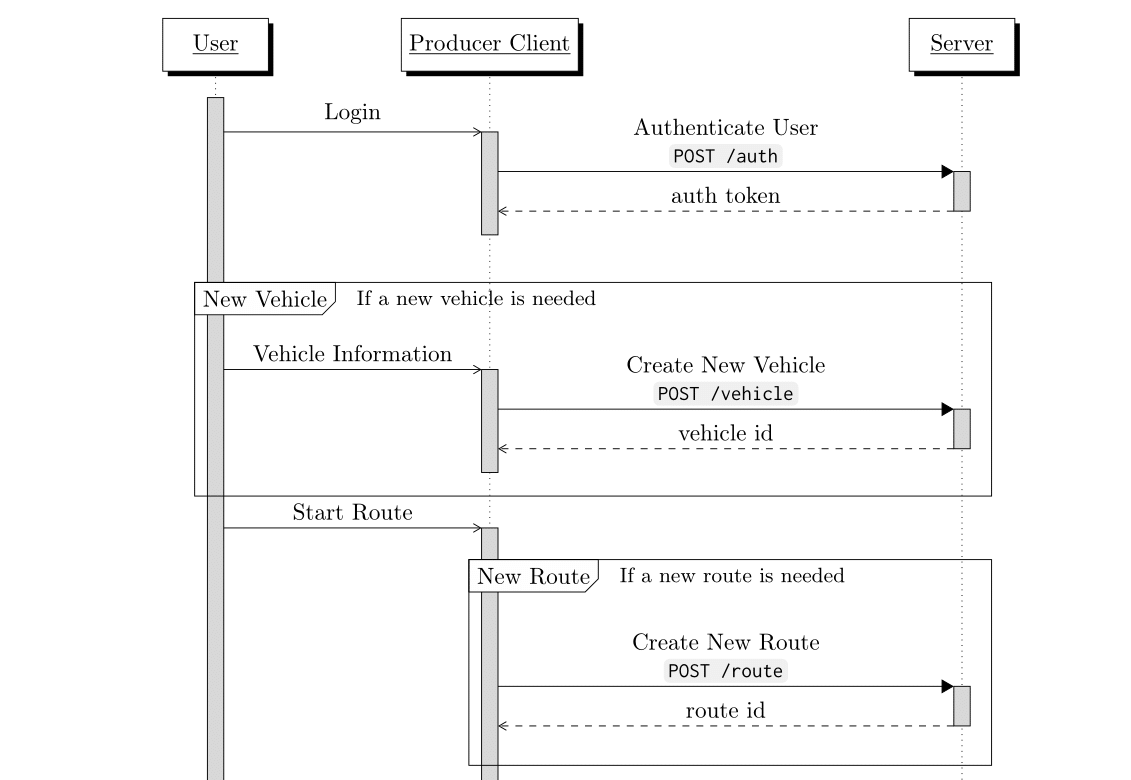
\includegraphics[width=1\textwidth]{imgs/top_seq.png}
        \end{figure}
    }
    \only<3| handout:3>{%
        \begin{figure}[htb]
            \centering
            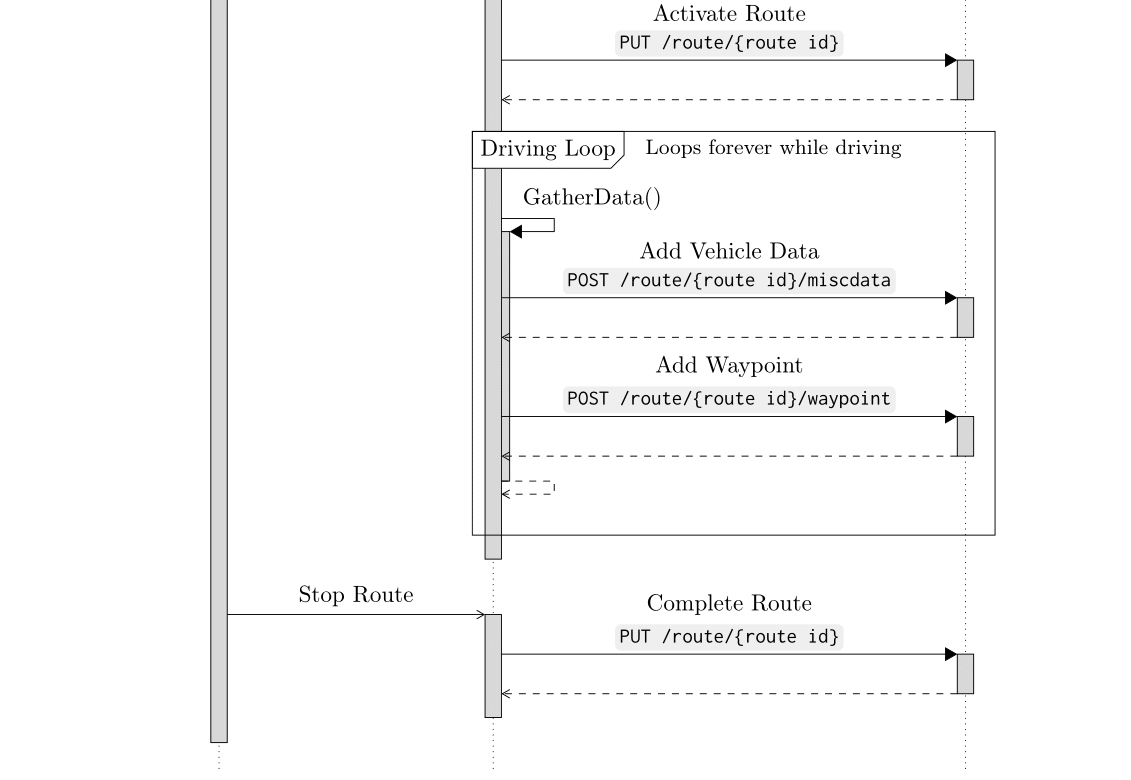
\includegraphics[width=1\textwidth]{imgs/bottom_seq.png}
        \end{figure}
    }
\end{frame}


\begin{frame}{System \& Load Testing}
    \framesubtitle{Testplan --- Fetching Data}
    Fetching data
    \begin{itemize}
        \item Simple fetching --- all users, all vehicles etc.
        \item Selective fetching --- all routes for a given driver
        \item Complex fetching --- \textbf{geospatial} queries
        \item \textbf{Normal load}: 100 fetching threads with 25 loops
        \item \textbf{Heavy load}: 400 fetching threads with 25 loops
    \end{itemize}
\end{frame}
